\section{Discussion \& Conclusion}
% motivation for creating this theme
\begin{frame}{Discussion}{}
    \begin{block}{Choice of ensemble factors}
    \begin{itemize}
        \item Object resolution clear
        \begin{itemize}
            \item MS COCO results, previous work
            \item Complements baseline 79.59 -> 80.09
        \end{itemize}
        \item IQA less clear
        \begin{itemize}
            \item More experimental choice
            \item Subjective IQA
            \item Distortions present in dataset?
        \end{itemize}
    \end{itemize}  
\end{block} 
\end{frame}

\begin{frame}{Discussion}{}
    \begin{block}{Object detector}
        \begin{itemize}
            \item R-FCN due to ResNet GPU requirements
            \item Method universal to detectors 
        \end{itemize} 
    \end{block} 
    \begin{block}{Creating data subsets}
        \begin{itemize}
            \item Heavily skewed in some cases
            \begin{itemize}
                \item Resolution, Gaussian blur
                \item Ensemble members different variance
            \end{itemize}
            \item Classes misrepresented in some ensemble members
        \end{itemize} 
    \end{block}
\end{frame}

\begin{frame}{Discussion}{}
\begin{columns}
    \column{0.5\textwidth}
        \begin{figure}
            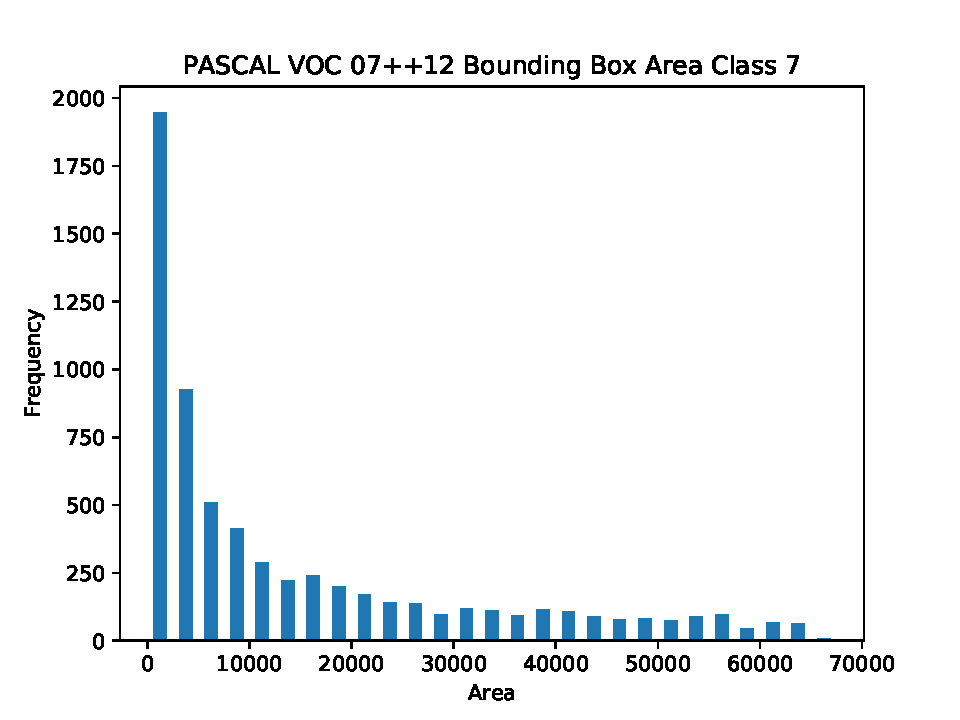
\includegraphics[width=1.0 \textwidth]{figs/trainvalhist_class7.pdf}
        \end{figure}
    \column{0.5\textwidth}
        \begin{figure}
            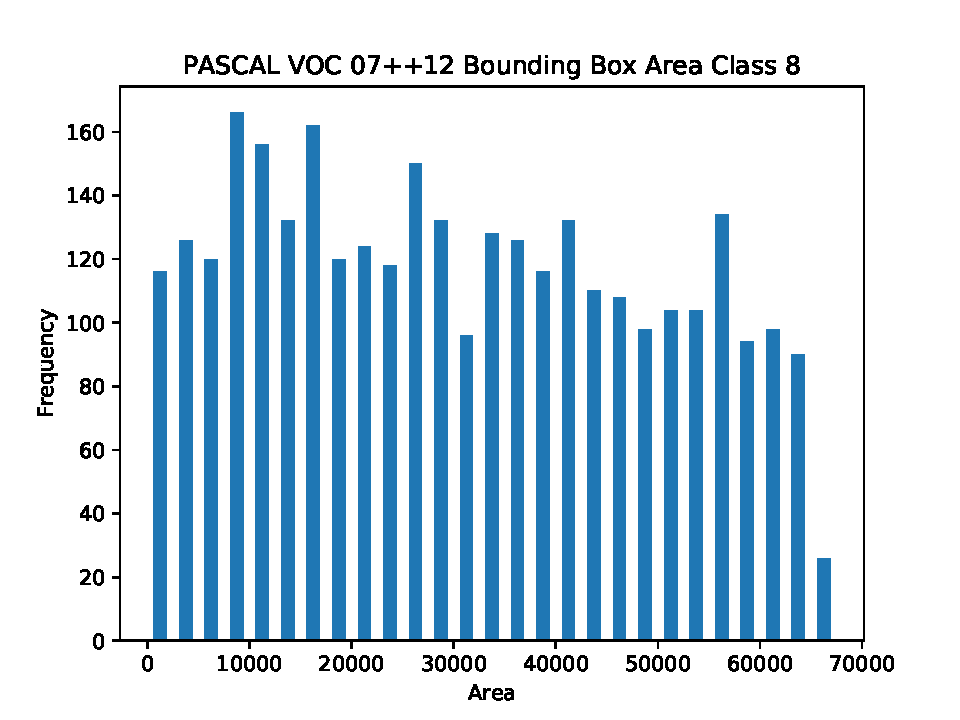
\includegraphics[width=1.0 \textwidth]{figs/trainvalhist_class8.pdf}
        \end{figure}
    \end{columns}
\end{frame}

\begin{frame}{Discussion}{}
    \begin{block}{Ensemble combination strategy}
        \begin{itemize}
            \item Factors members prefer different strategies
            \begin{itemize}
                \item Resolution -> Average
                \item IQA -> Weighted Average
            \end{itemize}
            \item Other methods possible?
            \begin{itemize}
                \item Boosting, bagging, stacking, etc
            \end{itemize} 
        \end{itemize} 
    \end{block} 
\end{frame}

\begin{frame}{Conclusion}{}
    \begin{block}{}
        \begin{itemize}
            \item Robustness-related challenges with a ensemble of R-FCNs
            \item Two ensemble strategies
            \begin{itemize}
                \item Data sampling and selection
                \item Ensemble combination
            \end{itemize}
            \item Multi-step training for R-FCN ensemble members
            \item Viable to engineer ensemble members towards object and image variations
            \item Conference article
        \end{itemize} 
    \end{block} 
\end{frame}